\documentclass{article}
\usepackage{graphicx} % Required for inserting images
\usepackage{hyperref}
\usepackage{listings}
\usepackage{subcaption}
\usepackage{multicol}
\usepackage[section]{placeins}
\usepackage{amsmath}
\usepackage{ragged2e}
\usepackage{dirtree}
\justifying

\title{Rezepti}

\author{ Christoph Sherr , Tobias Lotz, Dominik Hummel }
\date{June 2023}

\begin{document}

\begin{figure}
    \centering
    
\includegraphics[scale=0.3]{Pictures/rezepti.png}
    \label{fig:sfig1}
\end{figure}
\maketitle

\pagebreak
\section{Kurzbeschreibung:}
Eine Seite Für Kochrezepte von verschiedenen Ländern all around the globe.

\section{Zielgruppe Nutzer und Beeinflusser:}
Unsere Zielgruppe sind alle Personen die Spaß am Kochen haben oder auf der Suche nach Rezepten sind.

Beeinflusser sind unsere Nutzer selbst, Firmen die eventuell Werbung schalten wollen oder Rezepte 
sponsern könnten. Auch Influencer aus dem Kochsegment könnten Beeinflusser sein.


\section{Funktionen}
\begin{multicols}{2}
    \begin{itemize}
        \item Rezepte Filtern
        \item Rezepte suchen
        \item Anmeldung/Registrierung
        \item Abmeldung
        \item Rezept erstellen
        \item Rezepte Endecken
        \item Administaroren Seite
        \item Responsive Design
        \item Intuitive Bedienbarkeit
        \item Erstellen von Tags und Zutaten
        \item Anzeigen von Nutzerprofilen
        \item Rezept Bilder
    \end{itemize}
\end{multicols}

\pagebreak
\section{Referenzdokument}
%(mit Zielen, Funktionsrahmen bzw. allg. Funktionsbeschreibung, Projektrahmen, Umsetzungsstrategie, Aufgaben und Zuständigkeiten)


Ziel war es, eine Plattform zu schaffen, auf der Rezepte weltweit ausgetauscht werden können. Jeder Nutzer soll mit Hilfe eines Accounts nach Rezepten suchen und eigene Rezepte veröffentlichen können.\\
\\
Die Nutzer sollen Accounts anlegen, Rezepte einsehen und neue Rezepte erstellen können.
Es soll auch möglich sein, Rezepte ohne Anmeldung anzusehen.
Es soll möglich sein, Rezepte nach Zutaten, Kategorien und anderen Merkmalen zu suchen.
Außerdem soll es einen Admin-Bereich geben, in dem die Seite verwaltet werden kann.
Die Seite sollte intuitiv bedienbar sein, unabhängig vom Endgerät des Nutzers.\\
\\
Der Projektrahmen bestand hauptsächlich aus der Planung, der Implementierung und der Dokumentation des Ergebnisses. Die Implementierung nahm die meiste Zeit in Anspruch, ging aber teilweise mit der Planung einher.\\
\\
Für die Implementierung war bereits bei der Planung klar, dass wir ein Versionskontrollsystem benötigen, wofür wir Git zusammen mit GitHub verwendeten, was uns auch bei der Planung half, da wir einen Backlog in Github Projects einrichten konnten.\\
\\
Wir entschieden uns, Docker Compose für unser Projekt zu verwenden, damit jeder eine lauffähige Entwicklungsumgebung hatte. So konnte die Entwicklungsumgebung einfach auf jeder Maschine identisch zum Laufen gebracht werden.
Dies war auch für die Synchronisation der Datenbank nützlich. So konnten wir beim Start eine gedumpte SQL Datenbank laden.
Für das Backend erstellten wir eine allgemeine Klasse, über die man in jeder PHP Datei auf die Datenbank zugreifen konnte. Für das Frontend haben wir zunächst Vanilla CSS verwendet.\\
\\
Die Verantwortlichkeiten wurden bereits in der Planung festgelegt:
Domme sollte sich hauptsächlich um das Frontend und das Design der Website kümmern,
Tobias sollte sich um das Backend und die Datenbank kümmern.
Christoph hatte die Aufgabe, den Überblick zu behalten und das Frontend mit dem Backend zu verbinden.\\

\pagebreak
\section{Komplettes Product-Backlog als Tabelle}
\begin{table}[hbt!]
\centering
\begin{tabular}{@{}|l|l|@{}}
\hline
Aufgabe                                                                 & Status    \\ \hline
Dokumentation                                                           & done      \\ 
Use local dependencies instead of CDN                                   & done      \\ 
AJAX                                                                    & done      \\ 
fix xss in search                                                       & done      \\ 
Benutzerverwaltung                                                      & done      \\ 
synchronized header and footer                                          & done      \\ 
logout                                                                  & done      \\ 
Docker environment for windows                                          & done      \\ 
Kurzbeschreibung                                                        & done      \\ 
user profile page                                                       & done      \\ 
Rezepte erstellen                                                       & done      \\ 
Startseite                                                              & done      \\ 
detail view                                                             & done      \\ 
Rezept search                                                           & done      \\ 
jquery ui integration                                                   & done      \\ 
jquery integration                                                      & done      \\ 
load shared html from central files as templates                        & done      \\ 
search for ingridients                                                  & done      \\ 
search for tags                                                         & done      \\ 
fix potential sql injections                                            & done      \\ 
redisign detail view to be fancy                                        & done      \\ 
implement basic search                                                  & done      \\ 
upload images to on creation                                            & done      \\ 
automate user creation for db                                           & done      \\ 
Referenzdokument                                                        & done      \\ 
fix website for firefox                                                 & done      \\ 
switch from vanilla css to bootstrap                                    & done      \\ 
store images in the upload directory                                    & done      \\ 
automatically load recipies from database                               & done      \\ 
add a favicon                                                           & done      \\ 
use font available on any system                                        & done      \\ 
data sanitisation                                                       & done      \\ 
password management                                                     & done      \\ 
admin section                                                           & done      \\ 
session management                                                      & done      \\ 
Database structure                                                      & done      \\ 
\hline
\end{tabular}
\caption{
Im Verlauf des Projektes haben wir die "Projects" Funktion von GitHub verwendet, welche u.a. ein Kanban Board zu organisation anbietet.
Dieses kann unter folgendem Link gefunden werden:  
\url{https://github.com/users/PlexSheep/projects/2}
}
\end{table}



\pagebreak
\section{Technologien/Requirements}

\begin{itemize}
    \item Clienttechnologie: 
    \begin{itemize}
        \item CSS
        \item JS
        \item jQuery
        \item jQuery Tagify
        \item jQueryUI
        \item Bootstrap 5.3
        \item HTML5
    \end{itemize}
    
    \item Servertechnologie: 
    \begin{itemize}
        \item PHP
        \item MariaDB (MySQL)
        \item NGINX
    \end{itemize}
    
    \item Funktionelle Vorgaben:
    \begin{itemize}
        \item Sessionverwaltung
            \begin{itemize}
                \item Wird in der common.php datei (l. 7) gestartet
                \item Session expire in (l.  9 - 17)
                \item Session Abfrage z.B: in \verb|admin.php| (l. 14-19)
            \end{itemize}
        \item Login-Logout; automatisches Logout nach bestimmter Zeit
            \begin{itemize}
                \item Session expire in \verb|common.php| (l.  9 - 17) 
            \end{itemize}
        \item Admin-Bereich mit Useraccount-Verwaltung
            \begin{itemize}
                \item In \verb|admin.php|
                \item Nutzerverwaltung in den JavaScript Funktionen 
            \end{itemize}
        \item Passwort-Verwaltung
            \begin{itemize}
                \item In \verb|admin.php| (l. 105-129)
            \end{itemize}
        \item Rechte-Verwaltung (Adminrechte-Userrechte)
            \begin{itemize}
                \item Die Rechteverwaltung wird hier mit in Sessionvariablen gespeicherten IDs 
                    geregelt. Z.B: in \verb|admin.php| (l. 14-19)
            \end{itemize}
        \item Dateneingaben client- und serverseitig prüfen (RegExp)
            \begin{itemize}
                \item Implementiert in common.php \verb|test_for_bad_chars|,\\
                    \verb|test_for_bad_chars_array|. 
                    Die Funktionen selbst sind in der datei \verb|common.php| (l. 341-345) 
                    und (l. 347-353) deklariert.
            \end{itemize}
            \pagebreak
        \item Datensatzmanipulation in SQL-Server\\
            (speichern; auslesen/ausgeben; bearbeiten; löschen)
            \begin{itemize}
            \item Implementiert an vielen Stellen im Projekt. Die Rezepte, welche auf der 
                Startseite augegeben werden, werden aus der Datenbank geladen.
            \item Ausgabe: \verb|featured_recipies| (l. 5-8 und mehr)
            \item Speichern: \verb|admin.php| (l. 137-149)
            \item Bearbeitung: \verb|admin.php| (l. 105-132)
            \item Löschung: \verb|admin.php| (l. 72-99)
            \end{itemize}
        \item Konfigurationsdaten via Konfigurationsdatei einlesen
            \begin{itemize}
                \item Eine Konfigurationsdatei wird mit ini realisiert (\verb|rezepti_config.ini|).
                    Diese wird in \verb|common.php| (l. 20-55) geladen und deren Daten verwendet.
            \end{itemize}
        \item Einbindung von jQuery und jQuery UI\
            \begin{itemize}
                \item JQery und JQuery UI werden in der \verb|admin.php| Datei verwendet, 
                    um z.B: einen Confirmation-Dialog zu realisieren, der den Nutzer fragt, 
                    ob eine aktion ausgefhrt werden soll, sowie auch um AJAX einzubinden.
            \end{itemize}
        \item Dynamische laden/nachladen mit Hilfe von AJAX
            \begin{itemize}
                \item Realisiert in \verb|admin.php| (siehe oben)
            \end{itemize}
        \item Meldungsfenster und Userbestätigungen mit jQuery und jQuery UI
            \begin{itemize}
                \item Realisiert in \verb|admin.php| (siehe oben)
            \end{itemize}
        \item Datenexport via JSON
            \begin{itemize}
                \item Realisiert in \verb|get_user_data.php|
            \end{itemize}
        \item Dynamische Menüstruktur mit responsive Webdesign
            \begin{itemize}
                \item Auf der gesammten Seite vorhanden
            \end{itemize}
    \end{itemize}
\end{itemize}

\subsection{Beschreibung der verwendeten APIs (Frontend)}
\begin{itemize}
    \item Bootstrap 5.3\\
        Allgemeines CSS Framework mit Grid System
    \item JQuery\\
        JavaScript Library für AJAX, event handling, Widgets
    \item JQuery-UI\\
        JavaScript Library basierent auf JQuery für Nutzerfreundliche Widgets und andere
        UI Anwendungen
    \item Tagify\\
        JavaScript Library für Eingabefelder von Tags
\end{itemize}
\label{tab:my_label}

\pagebreak
\section{Verzeichnisstruktur}
Das Projekt hat mehrere Verzeichnisse, die nur für das Setup der Dockercontainer relevant sind. 
Diese sind die \verb|nginx|, \verb|php|, \verb|site|.conf und \verb|dev| Verzeichnisse. 
Die Verzeichnisse \verb|abgabe| und \verb|Documentation| sind nur Dokumentation.\\\\
Der eigentliche Code der Webapp befindet sich im Verzeichnis \verb|webdir|. 
In den in Webdir enthaltenen Unterordnern \verb|admin|, \verb|auth|, und \verb|templates| werden 
jeweils die Dateien für die Administarorenseiten, Authentifizierung und Templates gespeichert.
\verb|static| enthält die Dependencies, die geladen werden müssen.
\\
\\
\dirtree{%
.1 \text{.}.
.2 abgabe.
.2 documentation.
.2 dev.
.3 docker\_mysql\_init.
.2 nginx.
.2 php.
.2 site.conf.
.2 webdir.
.3 admin.
.3 auth.
.3 img.
.4 backgrounds.
.4 favicon.
.4 foods.
.4 icons.
.4 useruploads.
.3 static.
.4 \text{bs5.3}.
.5 \dots.
.4 \text{jquery-3.6.0}.
.5 \dots.
.4 \text{jquery-ui-1.13.2}.
.5 \dots.
.4 \text{tagify}.
.5 \dots.
.3 templates.
.3 test.
}

%\begin{figure}[!hbt]
%    \centering
%    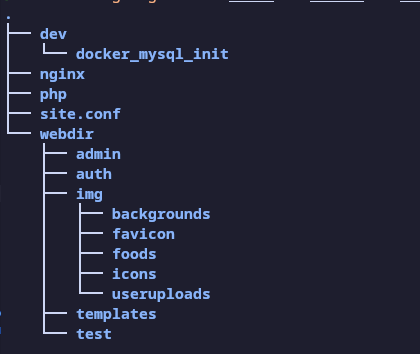
\includegraphics[scale=0.75, width=\textwidth]{Pictures/Dirs1.png}
%    \caption{Directories}
%    \label{fig:sfig1}
%\end{figure}


\pagebreak
\section{Beschreibung der Datenstrukturen \newline und Tabellen}

Für die Datenbank wurde nach Vorgabe MariDB verwendet. Diese Datenbank wurde in einem Dockercontainer gehostet und dann zur Bereitstellung der Daten angebunden.

\begin{figure}[!hbt]
    \centering
    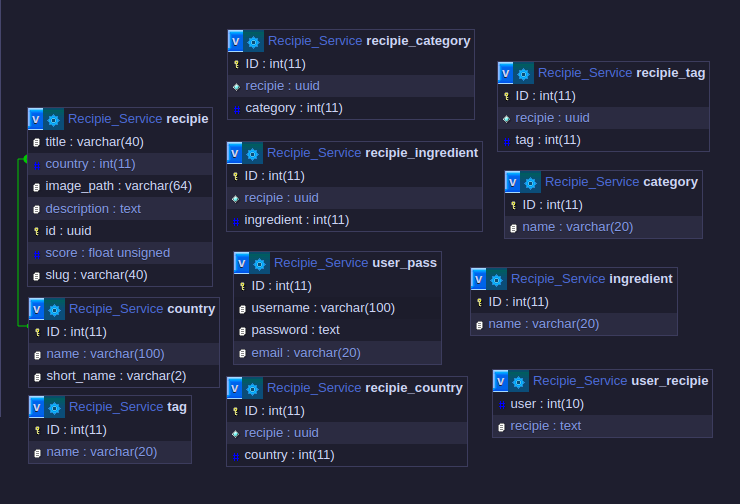
\includegraphics[scale=0.75, width=\textwidth]{Pictures/DB_Tables2.png}
    \caption{Datenbank Tabellen}
    \label{fig:sfig1}
\end{figure}

\subsection{recipie}
Haupttabelle der Rezepte
\newline
title: Titel des Rezepts
\newline
country: Land das dem Rezept zugewiesen wurde
\newline
image\_path: ID des Bildes, welchen in der webdir/img gespeichert werden.
\newline
description: Beschreibung des Rezeptes
\newline
id: uuid des Rezeptes
\newline
score: Bewertung des Rezeptes (Nicht genutzt)
\newline
slug: Referenzierung in der URL

\pagebreak

\subsection{country}
Tabelle für die Länder
\newline
ID: ID des Landes
\newline
name: Name des Landes
\newline
short\_name: Landeskürzel

\subsection{tag}
Tabelle für Tags
\newline
ID: ID des Tags
\newline
name: Name des Tags

\subsection{recipie\_category}
Verbindngstabelle für Rezepte und Länder
\newline
ID: Primary key
\newline
recipie: ID des Rezeptes
\newline
category: ID der Kategorie

\subsection{recipie\_ingridient}
Verbindngstabelle für Rezepte und Zutaten
\newline
ID: Primary key
\newline
recipie: ID des Rezeptes
\newline
ingidient: ID der Zutat

\subsection{user\_pass}
Tabelle für die Core Userdaten
\newline
ID: ID der User
\newline
username: Nutzername der User
\newline
password: Passwort der Nutzer
\newline
email: Email der Nutzer

\subsection{recipie\_country}
Verbindngstabelle für Rezepte und Länder
\newline
ID: Primary key
\newline
recipie: ID des Rezeptes
\newline
country: ID des Landes

\subsection{recipie\_tag}
Verbindngstabelle für Rezepte und Tags
\newline
ID: Primary key
\newline
recipie: ID des Rezeptes
\newline
tag: ID des Tags

\subsection{category}
Tabelle für die Kategorieen
\newline
ID: Primary key
\newline
recipie: ID des Rezeptes
\newline
name: Name der Kategorie

\subsection{ingidient}
Tabelle für die Zutaten
\newline
ID: Primary key
\newline
recipie: ID des Rezeptes
\newline
name: Name der Zutat

\subsection{user\_recipie}
Verbindngstabelle für User und Rezepte
\newline
user: ID des Users
\newline
recipie: ID des Rezeptes

\pagebreak

\section{Aufbau und Bedienbarkeit}
Rezepti zeichnet sich durch ein modernes Design und eine intuitive Benutzeroberfläche aus, die es Benutzern ermöglicht, Rezepte aus der ganzen Welt zu entdecken, zu teilen und zu speichern.

\subsection{Design und Layout}
Das Design der Web-App ist modern und benutzerfreundlich. Die Struktur der Web-App ist klar und übersichtlich, mit einer Navigationsleiste, die den Benutzern einen schnellen Zugriff auf die Hauptfunktionen der App ermöglicht. Auf der Startseite werden empfohlene Rezepte angezeigt, auf die die Benutzer mit einem einzigen Klick zugreifen können.

\subsection{Funktionalität}
Die Web-App bietet eine Vielzahl von Funktionen, die über die Benutzeroberfläche zugänglich sind. Benutzer können alle Rezepte einsehen und sich diese in einer Detailansiche genauer betrachten. Wenn sie Rezepte erstellen möchten, muss zuerst ein Konto auf der Seite angelegt werden. Nach der Anmeldung können sie auf ihre Profilseite zugreifen, auf der alle von ihnen  erstellten Rezepte angezeigt werden.  Die Suche nach Rezepten ist einfach und vielseitig, mit der Möglichkeit, nach Begriffen, Kategorien, Zutaten oder Länderkategorien zu suchen.

\subsection{Responsivität}
Die Web-App ist responsiv und passt sich an verschiedene Bildschirmgrößen an, einschließlich Desktop, Tablet und Handy. Dies gewährleistet eine konsistente Benutzererfahrung über verschiedene Geräte hinweg.

\end{document}
